\section{Opgave 1 -Simple procedure and function}
\begin{enumerate}
	\item[1)]
	
	Vi vil i denne opgave skrive VHDL-koden til komponenten illustreret på figur \ref{fig:component}
	\begin{figure}[h]
		\centering
		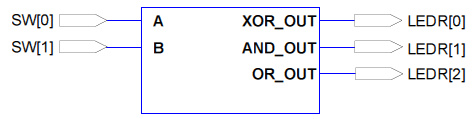
\includegraphics[scale=0.9]{pictures/Oevelse8/opg1/components}
		\caption{Komponent for simpel procedure og funktion}
		\label{fig:component}
	\end{figure}
	
	VHDL-koden for programmet er følgende:
	
\begin{lstlisting}[caption={Kode for simple procedure and function},label={lst:opg1_1}]
library ieee;
use ieee.std_logic_1164.all;

entity Exercise8_1 is
port (A, B: in std_logic ;
XOR_out, AND_out, OR_out : out std_logic);
end Exercise8_1;

architecture Mixed of Exercise8_1 is

function func_XOR (A : std_logic ; B : std_logic)return std_logic is
begin 
return (A xor B);
end func_XOR;

procedure proc_and_or (A, B : in Std_logic ; signal AND_out, OR_out : out std_logic) 
is 
begin 
AND_out <= (A and B);
OR_out <= (A or B);
end proc_and_or;

begin 
XOR_out <= func_XOR(A,B);
proc_and_or(A,B, AND_out, OR_out);

end Mixed;
\end{lstlisting}

\item[2)]
Vi overfører programmet til DE2-boardet, hvorpå der er pin-assignet som vist på figur \ref{fig:component}. Dette giver følgende resultater:

	\begin{figure}[h]
		\centering
		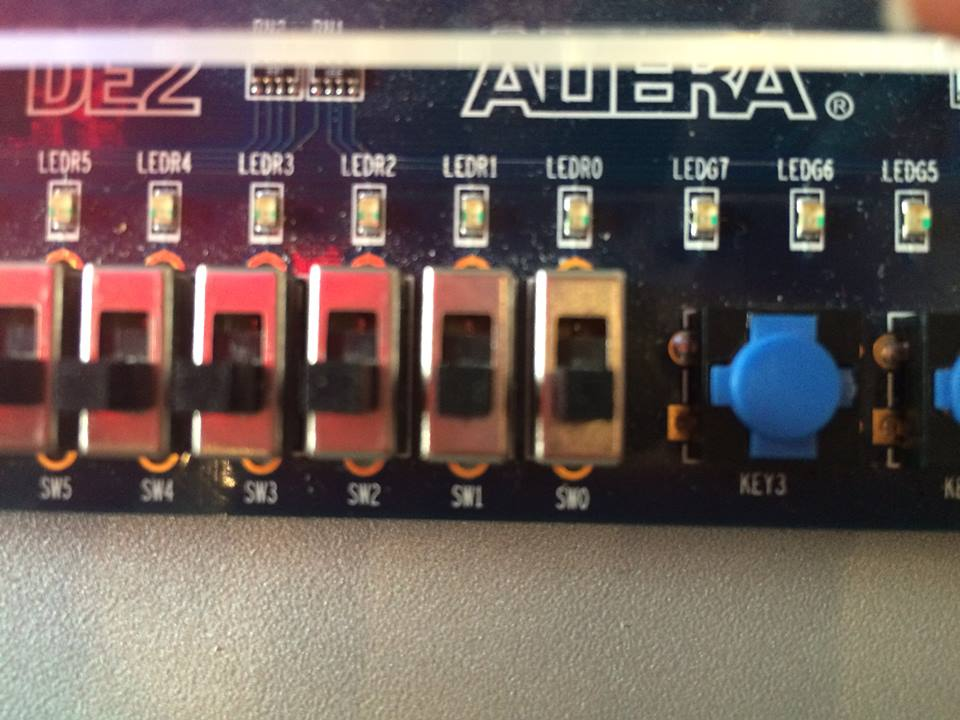
\includegraphics[scale=0.6]{pictures/Oevelse8/opg1/Function0_0}
		\caption{Inputs A og B er begge lave}
		\label{fig:figur0_0}
	\end{figure}

	\begin{figure}[h]
		\centering
		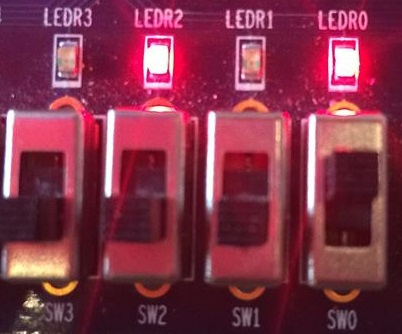
\includegraphics[scale=0.7]{pictures/Oevelse8/opg1/Function0_1}
		\caption{Input A er høj og B er lav}
		\label{fig:figur0_1}
	\end{figure}

	\begin{figure}[h]
		\centering
		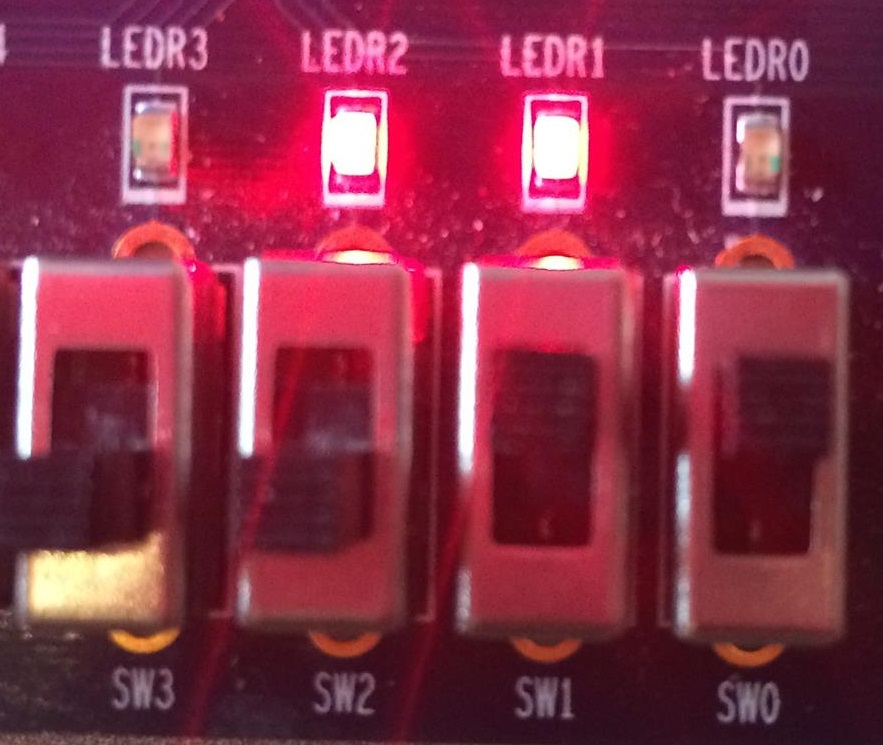
\includegraphics[scale=0.4]{pictures/Oevelse8/opg1/Function1_1}
		\caption{Inputs A og B er begge høje}
		\label{fig:figur1_1}
	\end{figure}
\clearpage

\item[2)]
Vi gemmer programmet som package på følgende måde:
\begin{lstlisting}[caption={Kode for package},label={lst:opg1_2}]
library ieee;
use ieee.std_logic_1164.all;

package Exercis8_2 is
function func_XOR (A : std_logic ; B : std_logic)return std_logic ;
procedure proc_and_or (A, B : in Std_logic ; signal AND_out, OR_out : out std_logic) ;
end Exercis8_2;

package body Exercis8_2 is
function func_XOR (A : std_logic ; B : std_logic)return std_logic 
is
begin 
return (A xor B);
end func_XOR;

procedure proc_and_or (A, B : in Std_logic ; signal AND_out, OR_out : out std_logic) 
is
begin 
AND_out <= (A and B);
OR_out <= (A or B);
end proc_and_or;

end Exercis8_2;
\end{lstlisting}

Denne package kan testes ved hjælp af følgende kode:

\begin{lstlisting}[caption={Kode for test af package},label={lst:opg1_2test}]
library ieee;
use ieee.std_logic_1164.all;
use work.exercis8_2.all;

entity Exercise8_2 is 
port ( A, B : in std_logic;
XOR_out, AND_out, OR_out : out std_logic);

end Exercise8_2;

architecture simplePackage of Exercise8_2 is

begin 
XOR_out<= func_XOR(A,B);
proc_and_or(A, B, AND_out, OR_out);

end simplePackage;

\end{lstlisting}

Vi overfører programmet til DE2-boardet og tester. Dette giver os, som forventet, samme resultat som vist på figur \ref{fig:figur0_0}, \ref{fig:figur0_1} og \ref{fig:figur1_1}.

\end{enumerate}